\rhead{16 Mai 2018}
\begin{proof}
\begin{enumerate}[(1)]
\item \begin{align*}
s_1&:=\#\{k \in \{1, \dots, n\} \ | \ p \text{ teilt } k \} = \lfloor \frac{n}{p} \rfloor = \sum_{i=1}^r a_i p^{i-1}\\
s_2&:=\#\{k \in \{1, \dots, n\} \ | \ p^2 \text{ teilt } k \} = \lfloor \frac{n}{p^2} \rfloor = \sum_{i=2}^r a_i p^{i-2}\\
\dots\\
s_1&:=\#\{k \in \{1, \dots, n\} \ | \ p^r \text{ teilt } k \} = \lfloor \frac{n}{p^r} \rfloor = a_r
\end{align*}
\item $v_p(n!)=s_1+s_2+\dots + s_r = a_1+a_2(1+p)+a_3(1+p+p^2)+\dots+a_r(1+p+\dots+p^{r-1})$\\
$(p-1)v_p(n!)=a_1(p-1)+a_2(p^3-1)+\dots+a_r(p^r-1) \Rightarrow$ Beh.
\end{enumerate}
\end{proof}

\begin{Lem}
Sei $K/\Q_p$ $p$-adischer Zahlkörper.\\
Dann gilt für $x \in K:$
\[\forall k \in \N: \hat v (\frac{x^k}{k!})=k(\hat v(x)-\frac{e}{p-1}) + \frac{e}{p-1}t_k\]
mit $t_k=a_0+a_1+\dots+a_r$ für $k=\sum_{i=0}^r a_i p^i$.
\end{Lem}

\begin{proof}
Lemma 7.14 $\Rightarrow \hat{v}(k!)= e v_p(k!)=\frac{e}{p-1}(k-t_k)$\\
$\Rightarrow \hat{v}(\frac{x^k}{k!})=k \hat{v}(x)-\hat{v}(k!)=k(\hat{v}(x)-\frac{e}{p-1})+\frac{e}{p-1}t_k$
\end{proof}

\begin{proof}[Beweis von Prop. 7.13]
$n>\frac{e}{p-1}$\\
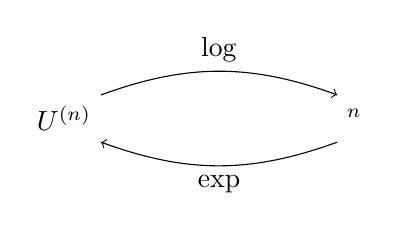
\begin{tikzpicture}[scale=3]
\node[left] at (0,0){$U^{(n)}$};
\node[right] at (1,0) {$\hP^n$};
\draw[->] (0,0.1) to [out=20, in=160] node[above]{$\log$} (1,0.1);
\draw[->] (1,-0.1) to[out=200, in=340] node[below]{$\exp$} (0,-0.1);
\end{tikzpicture}
\begin{enumerate}[(1)]
\item \underline{Zeige:} $\sum_{k=0}^\infty \frac{x^k}{k!}$ konvergent für $x \in \hP^n$ mit $n>\frac{e}{p-1}$\\
Lemma 7.16 $\Rightarrow \hat{v}(\frac{x^k}{k!})>\frac{e}{p-1}t_k$, da $\hat{v}(x) \geq n > \frac{e}{p-1} \Rightarrow \hat{v}(\frac{x^k}{k!}) \to \infty$
\item \underline{Zeige:} $\exp(x)=\sum_{k=0}^\infty \frac{x^k}{k!} \in U^{(n)} = 1+\hP^n$ für $x \in \hP^n$.\\
Zeige dazu: $\hat{v}(\exp(x)-1)=\hat{v}(x)$ und somit $\exp(x)-1 \in \hP^n.$\\
Für $k\geq 2: \hat{v}(\frac{x^k}{k!}) \stackrel{\text{Lemma 7.16}}{=\joinrel =} (k-1) \hat{v}(x)+\frac{e}{p-1}\underbrace{(t_k-k)}_{=t_k-1+1-k}+\hat{v}(x)\\
=\underbrace{(k-1)\hat{v(x)}}_{>(k-1)\frac{e}{p-1}}-(k-1)\frac{e}{p-1}+ \underbrace{(t_k-1)\frac{e}{p-1}}_{>0} + \hat{v}(x)>\hat{v}(x)$\\
$\stackrel{\Delta-\text{Ungl.}}{\Rightarrow} \hat{v}(\exp(x)-1)=\hat{v}(x) \geq n \Rightarrow \exp(x) \in U^{(n)}.$
\item \underline{Zeige:} $1+z\in U^{(n)} \Rightarrow \log(1+z)\in \hP^n$.\\
$z\in \hP^n \Rightarrow \hat{v}(z) \geq n > \frac{e}{p-1}.$\\
Für $k \geq 2: \hat{v}(\frac{z^k}{k})-\hat{v}(z) = k \hat{v}(z) - \hat{v}(z) - \underbrace{\hat{v}(k)}_{\leq \frac{k-1}{p-1}e} \stackrel{\text{Lemma 7.14}}{\geq} (k-1)\hat{v}(z) - \frac{k-1}{p-1}e >0$.\\
Beh. folgt analog wie in (2).
\item Stetigkeit folgt aus Lemma 7.17.
\item $\log$ und $\exp$ sind invers zueinander (Nachrechnen für formale Potenzreihen).
\end{enumerate}
\end{proof}

\begin{Lem}
Sei $K$ nicht-archimedischer Körper mit Bewertung $v$ und $\sum_{k \geq 0} a_k X^k$ Potenzreihe mit $a_k \in K$.\\
Ist $\mathbb{D}=\{x \in \O^\times \ | \ \sum_{k \geq 0} a_k x^k \text{ ist konvergent} \}$, dann ist die Abbildung $\mathbb{D} \to K \ , \ x \mapsto \sum_{k\geq 0} a_k x^k$ stetig.
\end{Lem}

\begin{proof}
Sei $x_n$ Folge in $\mathbb{D}$ mit $x_n \to x \in \mathbb{D}$. Zeige also: $\sum_{k \geq 0} a_k x^k_n \to \sum_{k \geq 0} a_k x^k$.\\
Wähle $n_0$ mit $v(x_n)=v(x) \ \forall n \geq n_0$.\\
Sei $N >0$ beliebig. $\sum_{k \geq 0} a_k x^k_n$ und $\sum_{k \geq 0} a_k x^k$ sind konvergent\\
$\Rightarrow |a_kx^k_n| \to 0$ und $|a_kx^k| \to 0$ für $k \to \infty$.\\
$\Rightarrow \exists k_0$ mit $v(a_kx^k) >N$ für $k \geq k_0$.\\
$\Rightarrow \forall n \geq n_0: v(a_nx_n^k)=v(a_nx^k)>N$\\
Betrachte $v(a_0), \dots, v(a_{k_0})$.\\
Sei $m:= \min\{v(a_0), \dots, v(a_{k_0})\}$. Wähle $n_1 \in \N$ mit $v(x-x_n)>N-m \forall n \geq n_1$.\\
Außerdem gilt: $v(x^k-x_n^k) \geq v(x-x_n)$ denn:\\
\[x^k=(x_n+(x-x_n))^k=x_n^k+(x-x_n) \cdot \underbrace{(\sum_{j=1}^k {k \choose j} x_n^{k-j} (x-x_n)^{j-1})}_{\in \O}.\]
Nun gilt für $v_n:=v(\sum_{k \geq 0} a_k x^k - \sum a_k x_n^k)=v(\sum_{k \geq 0} (x^k-x^k_n))$, falls $n \geq n_0, n_1$, dann:
\begin{itemize}
\item $v(a_k(x^k-x_n^k)) \geq \min \{v(a_kx^k), v(a_kx_n^k)\} \geq N$ für $k \geq k_0$
\item $v(a_k(x^k-x_n^k)) \geq v(a_k)+v(x-x_n) \geq m +N - m =N$ für $k \leq k_0$
\end{itemize} 
$\Rightarrow v_n \geq N$ für $n \geq n_0, n_1 \Rightarrow$ Beh.
\end{proof}

\begin{Bem}
Sei $K$ lokaler Körper mit $\ch(\hat{\kappa})=p$. Dann hat $U^{(1)}$ natürliche Struktur als $\Z_p$-Modul.
\begin{enumerate}[i)]
\item $U^{(1)}=\limproj_n U^{(1)}/U^{(n+1)}$, da $U^{(1)}$ abgeschlossen in $K$ und $K$ vollständig.\\
$U^{(1)} \supset U^{(2)} \supset U^{(3)} \supset \dots$.\\
$\Z_p \cong \limproj_{n \in \N} \Z/p^n\Z \cong \limproj_{n \in \N} \Z/q^n\Z$ für $q:=\#\hat{\kappa}$.
\item Es gilt: $\underbrace{U^{(n)}/U^{(n+1)} \cong \hP^n/\hP^{n+1}}_{1+x \mapsfrom x} \cong \hO / \hP \cong \hat{\kappa}$\\
$\Rightarrow U^{(1)}/U^{(n+1})$ ist abelsche Gruppe mit $q^n$ Elementen.\\
$\Rightarrow$ Erhalte Struktur als $\Z/q^n\Z$-Modul durch:
\[\Z/q^n\Z \times U^{(1)}/U^{(n+1)} \to U^{(1)}/U^{(n+1)} \ , \ (\bar{k}, \overline{1+x}) \mapsto \overline{(1+x)^k}\]
\item Die Multiplikationen aus ii) kommutieren mit Projektionen ($m \leq n$):
\[\begin{tikzcd}
\Z/q^n\Z \times U^{(1)}/U^{(n+1)} \arrow[r] \arrow[d] & U^{(1)}/U^{(n+1)} \arrow[d]\\
\Z/q^m\Z \times U^{(1)}/U^{(m+1)} \arrow[r] &U^{(1)}/U^{(m+1)}
\end{tikzcd}\]
$\Rightarrow$ Erhalte auf $U^{(1)}= \limproj U^{(1)}/U^{(n+1)}$ Struktur als $\Z_p$-Modul.\\ Insbesondere gilt: $z_i \in \Z \to z \in \Z_p \Rightarrow (1+x)^{z_i} \to (1+x)^z$ für $x \in \hP$.
\end{enumerate}
\end{Bem}
